\documentclass[12pt]{article}
\usepackage[english]{babel}
\usepackage{natbib}
\usepackage{url}
\usepackage[utf8x]{inputenc}
\usepackage{amsmath}
\usepackage{graphicx}
\usepackage{subfigure}
\graphicspath{{images/}}
\usepackage{parskip}
\usepackage{fancyhdr}
\usepackage{vmargin}
\usepackage{float}
\usepackage[none]{hyphenat}
\setmarginsrb{3 cm}{2.5 cm}{3 cm}{2.5 cm}{1 cm}{1.5 cm}{1 cm}{1.5 cm}

\title{Image Classification for Fashion Products}								% Title
\author{}			% Author
\date{Spring ’2017-2018}											% Date

\makeatletter
\let\thetitle\@title
\let\theauthor\@author
\let\thedate\@date
\makeatother

\pagestyle{fancy}
\fancyhf{}
\lhead{\thetitle}
\cfoot{\thepage}

\begin{document}

%%%%%%%%%%%%%%%%%%%%%%%%%%%%%%%%%%%%%%%%%%%%%%%%%%%%%%%%%%%%%%%%%%%%%%%%%%%%%%%%%%%%%%%%%

\begin{titlepage}
	\centering
    \vspace*{0.5 cm}
    
    
\includegraphics[scale = 0.3]{hu_logo.png}\\[1.2 cm]
	\textsc{\Large BBM 416}\\[0.5 cm]
	\textsc{\large Computer Vision}\\[2 cm]
    
	{ \huge \bfseries \thetitle}\\
	\rule{\linewidth}{0.2 mm} \\[1.5 cm]
	
    \emph{Authors:} \\ [0.5 cm]
    Didem ÖZTEKİN - 21328361 \\ [0.4 cm]
    Meral Büşra TEKİNŞEN - 21328485 \\ [0.4 cm]
    Yılmaz BAYSAL - 21327694 \\ [4 cm]
	
    {\large \thedate}\\[2 cm]
\end{titlepage}

\pagebreak

%%%%%%%%%%%%%%%%%%%%%%%%%%%%%%%%%%%%%%%%%%%%%%%%%%%%%%%%%%%%%%%%%%%%%%%%%%%%%%%%%%%%%%%%%

\tableofcontents
\pagebreak

%%%%%%%%%%%%%%%%%%%%%%%%%%%%%%%%%%%%%%%%%%%%%%%%%%%%%%%%%%%%%%%%%%%%%%%%%%%%%%%%%%%%%%%%%

\section{Problem Definition}

The aim of the project is to classify the fashion products by training the dataset given by the “Kaggle” and build models that perform labeling operation for fashion products.\\
	\\The dataset consists of approximately 25000 images with several attribute labels. A json file, which includes the image id, url to download image and attribute labels(for training set), is provided for the training and test sets. Thanks to the algorithm is developed, the links in the train data set are downloaded and each image is multi-tagged.\\
	\\After this labeling, the features of the pictures are extracted and these features are trained, tested and each image is classified. The expected output format is test image ids and theirs classified labels. 


\section{Methods And Algorithm}

\subsection{Dataset Loading and Parsing}
The given train dataset contains links of images, ids, and multiple labels for these images. Similarly, the given test dataset contains links of images and ids. For this reason, these images had to be downloaded by using these links first. To achieve this, we have used a code which was implemented by another competitor on Kaggle Discussion page and modified this code according to our problem.  After downloading the images,  they were named so as to keep the image ID and the tags for training dataset. (For example, imageid\_123[2,3,4,5].jpg, in here the tags are the numbers shown in parentheses.). The files were put into a train folder by using this naming standard.\\
 \\Also, the labels were put in a list with the making necessary splittings to hold the labels for each image by using regular expressions. After defined labels listed for each image, a bag of words which contains all labels was created. The labels lists and bag of words were compared each other, if the label which is in bag of word is in the labels list one was written, otherwise zero is written. In this way, a binary label lists was created for each image.


\subsection{Feature Extraction}
In machine learning and image processing, the first step of almost all algorithms is extracting the features from the data. These features represent our data with smaller memory usage in the system.\\
\\Spatial feature is a virtual representation of layout that is most commonly classified as a point, line, or polygon. It also  include the information about coordinates, intensity, gradient, resolution.\\
\\In our dataset, we decided to extract the spatial features for each image with using a CNN architecture. We generated a pre-trained VGG16 model by using keras library that is a neural network API developed with Python. We perform feature extraction from the pre-last layer and reshaped the results as 4096x1 vector.\\


The architecture of VGG16\: the input layer takes an image in the size of (224 x 224 x 3), and the output layer is a softmax prediction on 1000 classes. From the input layer to the last max pooling layer (labeled by 7 x 7 x 512) is regarded as the feature extraction part of the model, while the rest of the network is regarded as the classification part of the model. To avoid trouble while training the spatial features, a spatial vectors which dimensions are 4096 is created by resizing the spatial matrix. 

\begin{figure}[H]
\centering
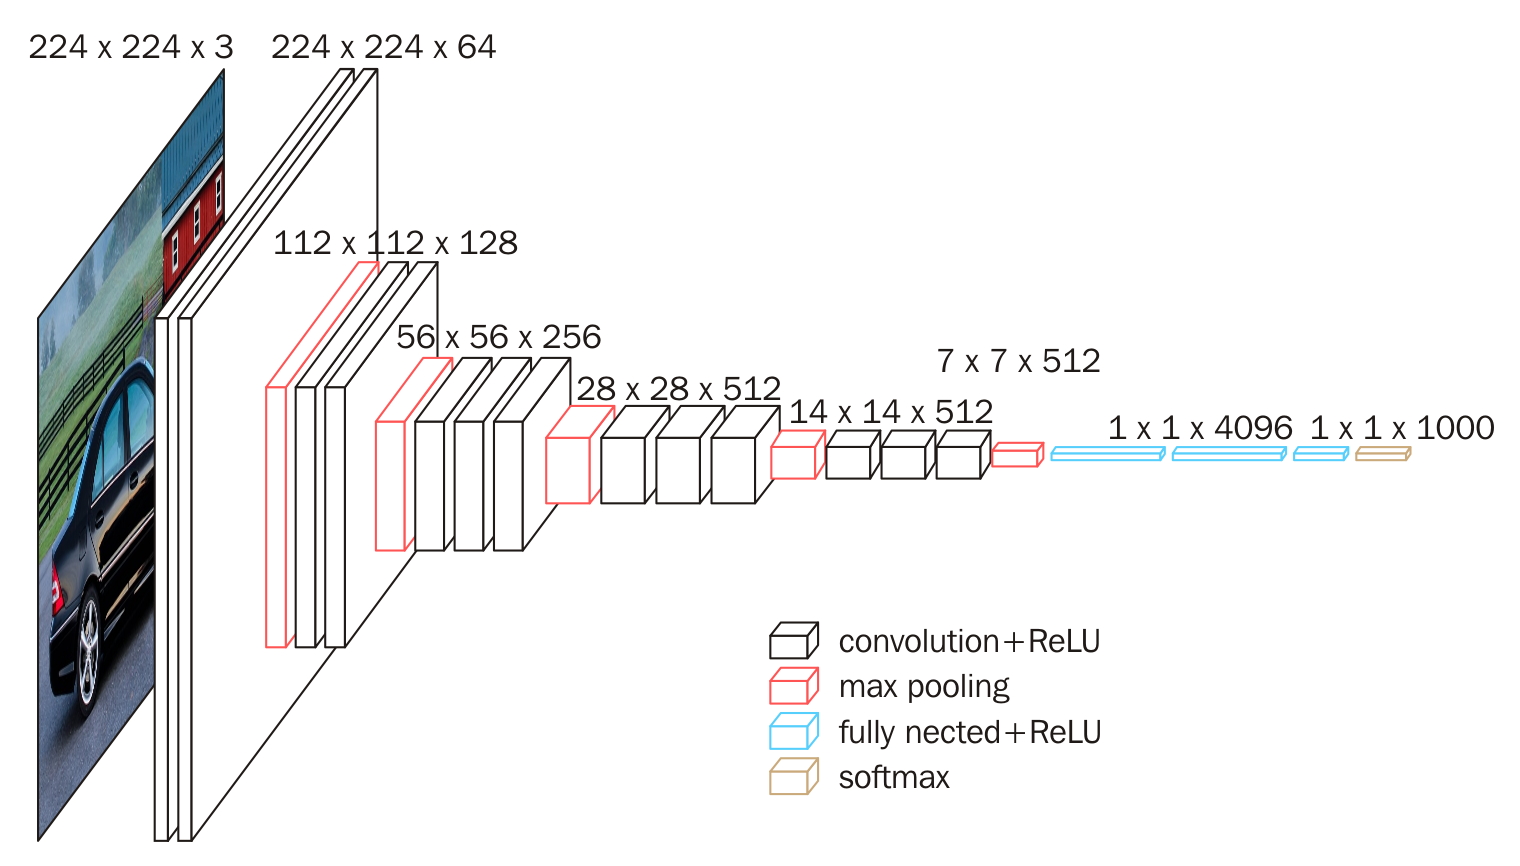
\includegraphics[width=.90\textwidth]{vgg16.png}
\caption{VGG16 Architecture}
\end{figure}

Since the number of data used in the project was very large, a csv file has been created and the vectors and tags corresponding to the images was printed to the train csv file. This operation saved both performance and memory space. The same procedure was applied for the test data set. A csv file has been created and the vectors corresponding to the images was printed to the test csv file. 



\subsection{Training}

In the training phase, we have to learn a model that is able to classify the vectors which is belong images in the csv train file and labels of images were trained. For that purpose, the simple Multi-layer Perceptron was implemented by using \textit{Keras}. 
 In multilayer perceptron, the model needs to know what input shape it should expect. For this reason, the first layer in a “Sequential” model (and only the first, because following layers can do automatic shape inference) needs to receive information about its input shape. So, we set the input shape for the model as 4096x1. Our multilayer perceptron implementation consists of 4 fully connected layers ( 1 input, 1 output and 2 hidden layers).\\
\\We also performed batch normalization on all layers and added one Dropout layer after the first hidden layer. Thus we prevented overfitting, made network train faster, converge much more quickly, try higher learning rates and get more accurate results.\\

Activation function was defined as “sigmoid” because when \textit{Softmax} and \textit{Sigmoid} compare to each other Sigmoid gave better results. 
The loss functions was defined “binary\_crossentropy” because bag of words that were used and list of labels of images was defined as binary list. For example, an image: the labels list of this image [1,0,0,1,1…] 1 is if the label in bag of word is in the label list of images otherwise is zero. 
The train data was shuffled to reduce memorization of pictures.

\begin{figure}[H]
\centering
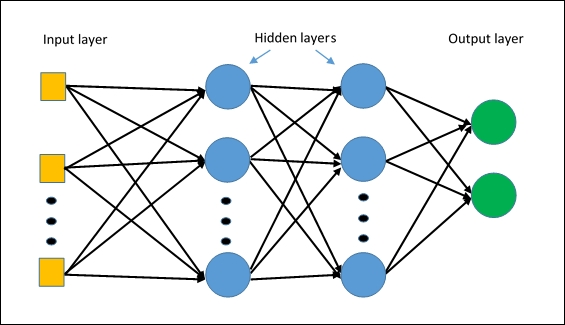
\includegraphics[width=.90\textwidth]{mlp.jpg}
\caption{Multi-Layer Perceptron Architecture}
\end{figure}

\subsection{Testing and Validation}

In training phase, we enabled self validation feature of the the model by only setting the \textit{validation\_split} attribute. We set this value as 0.1 so, the 10\% of the train images will be used to validate the model.

In testing phase, the model generated output predictions for the input samples. Computation was done in batches. As the result, probability of each label was calculated for each image. The ID of images, their most probable label and over 50\% labels was printed to a CSV file. Finally, we uploaded the output file to the \textit{kaggle} website and calculated got the textit{mean-f1} score.

\section{Results}

The application that we created generates classification results as a CSV file and also plots the training and the validation metrics (loss and accuracy) to the screen. On the below figure, you can see a sample image with the assigned labels. \\

\begin{figure}[H]
\centering
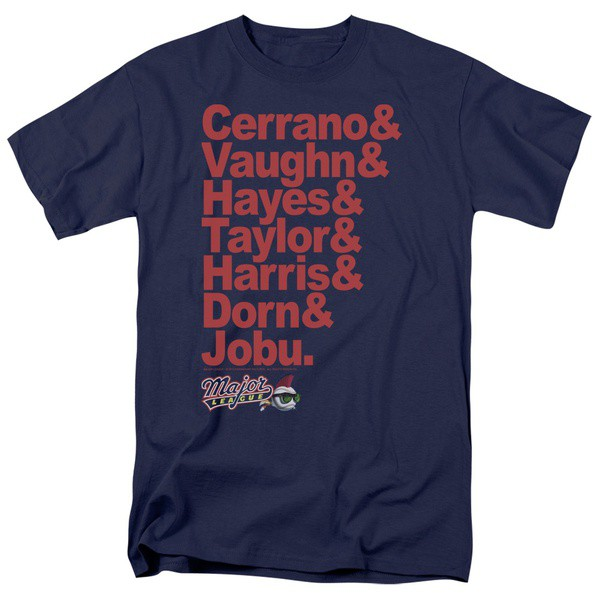
\includegraphics[width=1\textwidth]{6103.jpg}
\caption{Test sample: 6103 - Predicted labels: [106, 153, 53, 164]}
\end{figure}

We tested our application with using different methods to achieve better results and more performance. Then, we chose the configuration with the highest mean-f1 score. You can see the results of these trials below.

\begin{figure}[H]
\centering
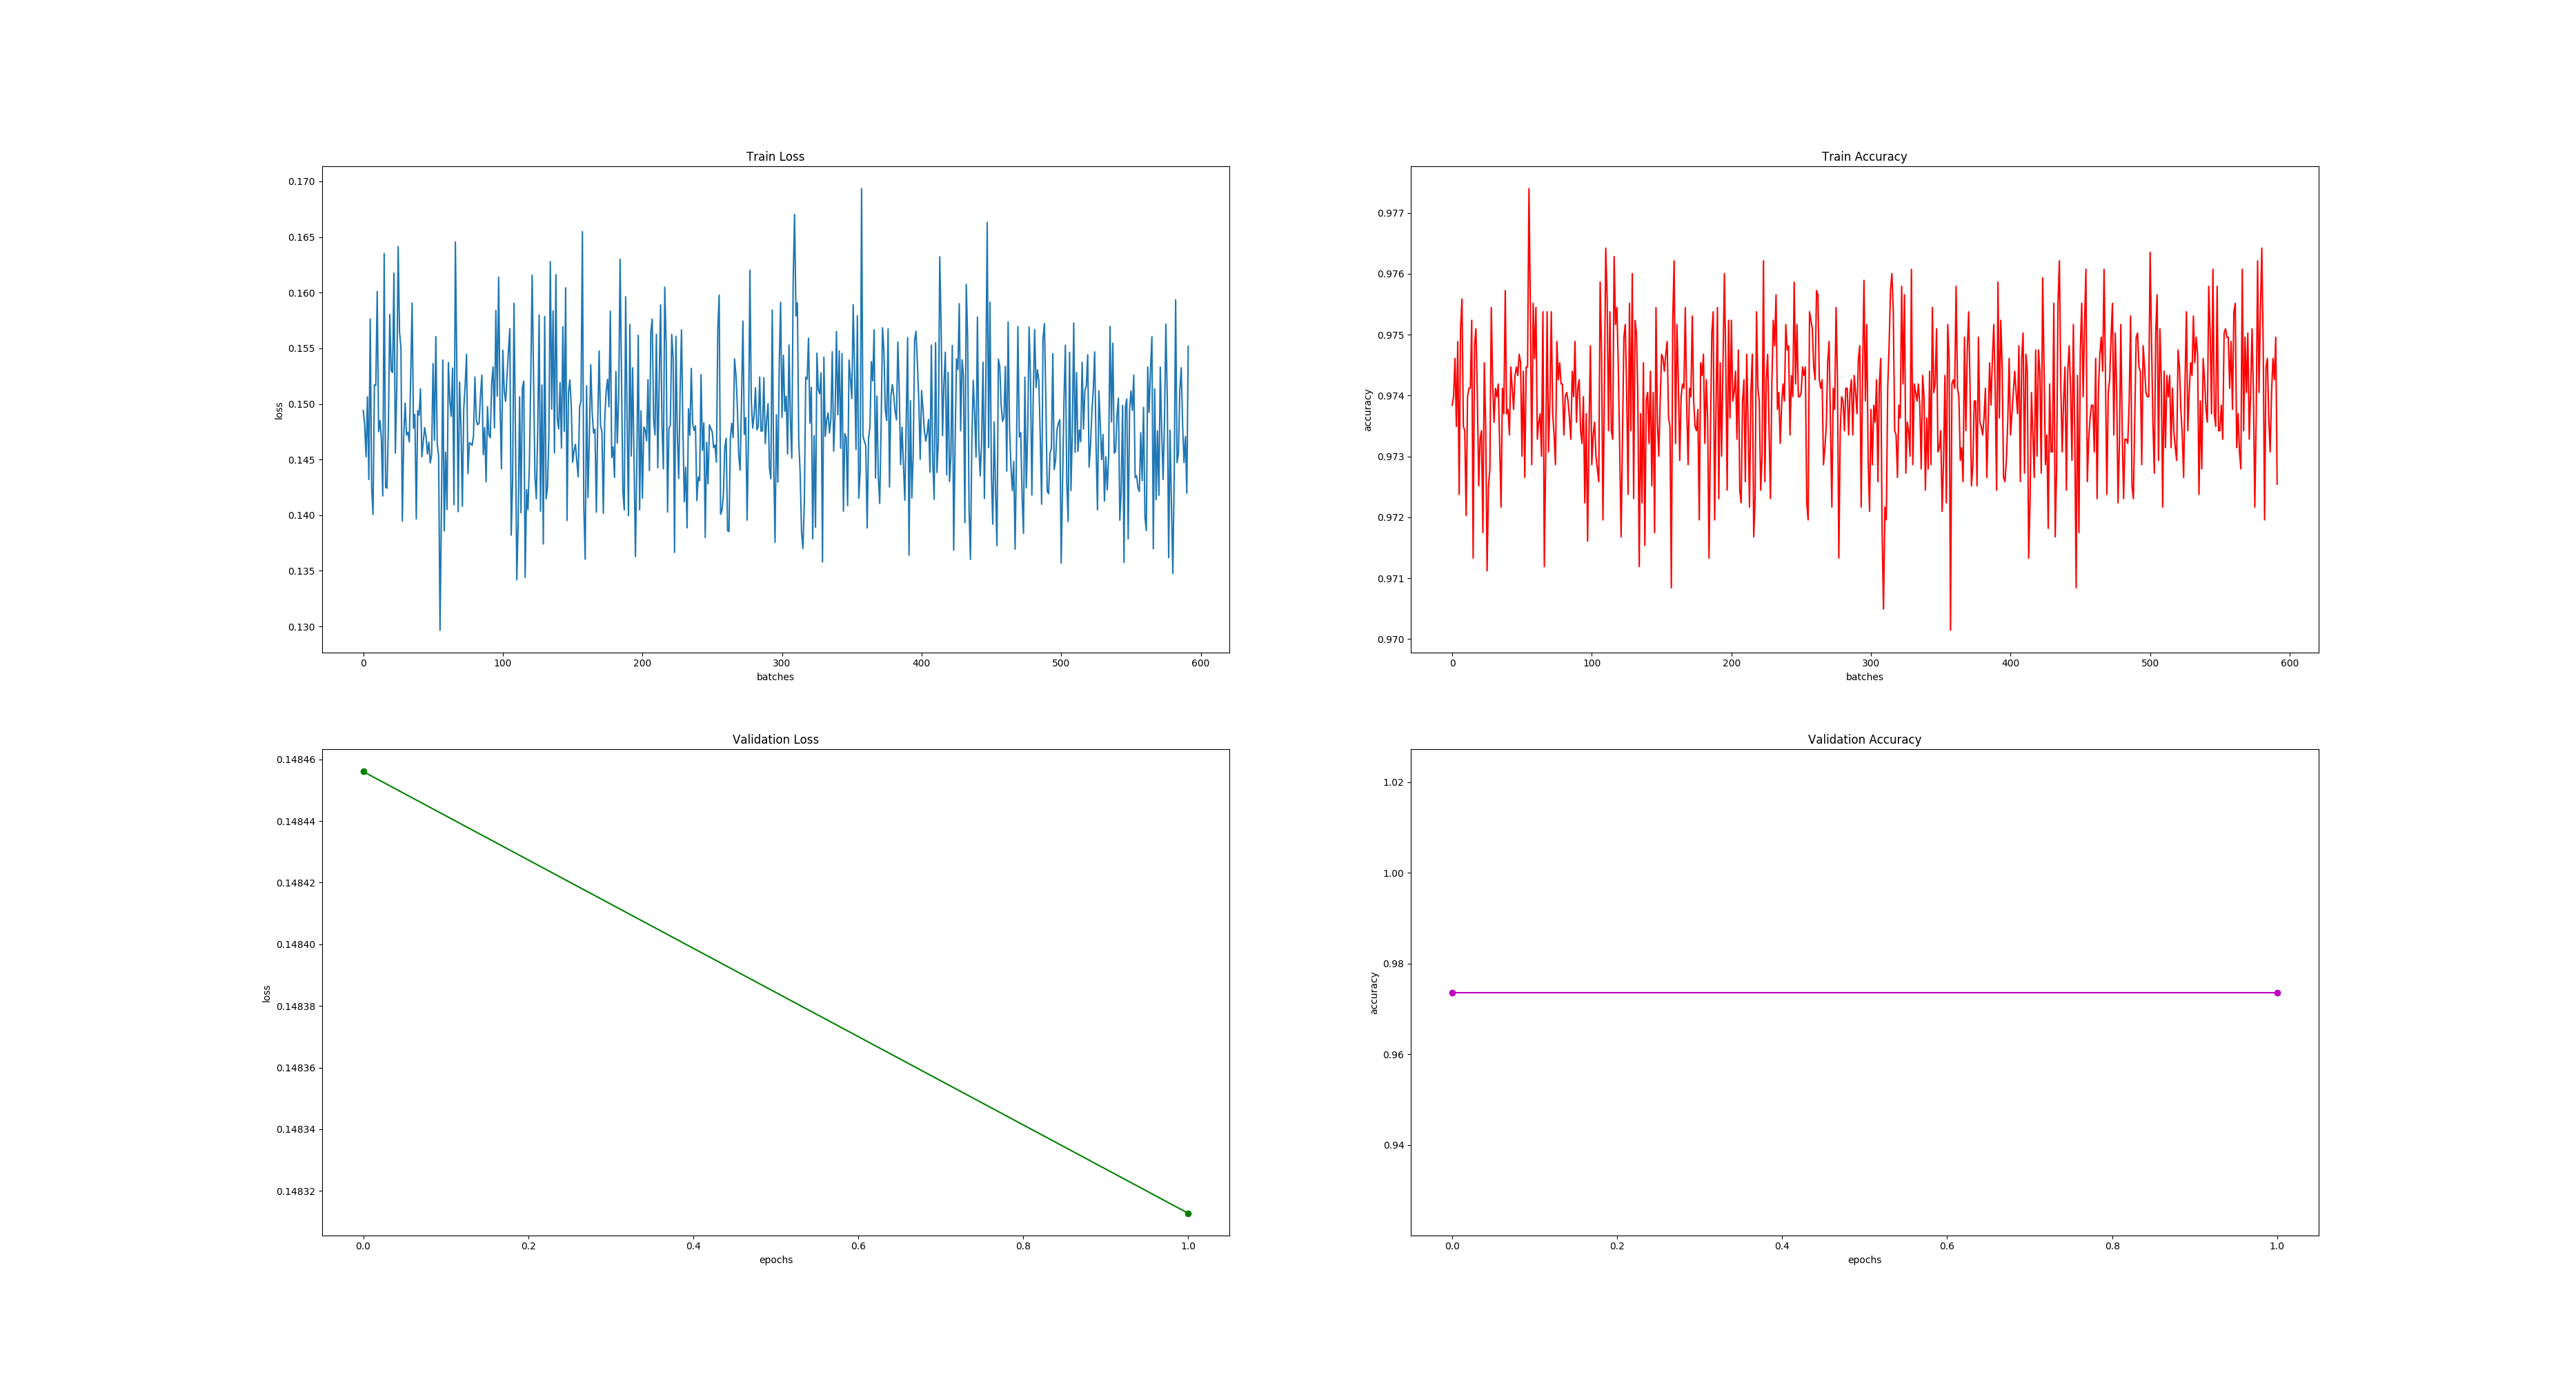
\includegraphics[width=1\textwidth]{2ep_64btch_softmax.png}
\caption{2 epochs, 64 batch-size, Softmax activation function, Adam optimizer}
\end{figure}

As can be seen on the above figure the training loss and the training accuracy lines bounces around a lot and the loss is not decreasing smoothly. Another problem with this configuration was the significant decrease of the probabilities. They were clustered around 10\% and we were not able to threshold them. So, we only get the max probable label. \\

The mean-f1 score of this configuration is 0.87999. It can be seen as a quite good result but, it is achieved by getting only the most probable labels. Other probable labels have been lost.

\begin{figure}[H]
\centering
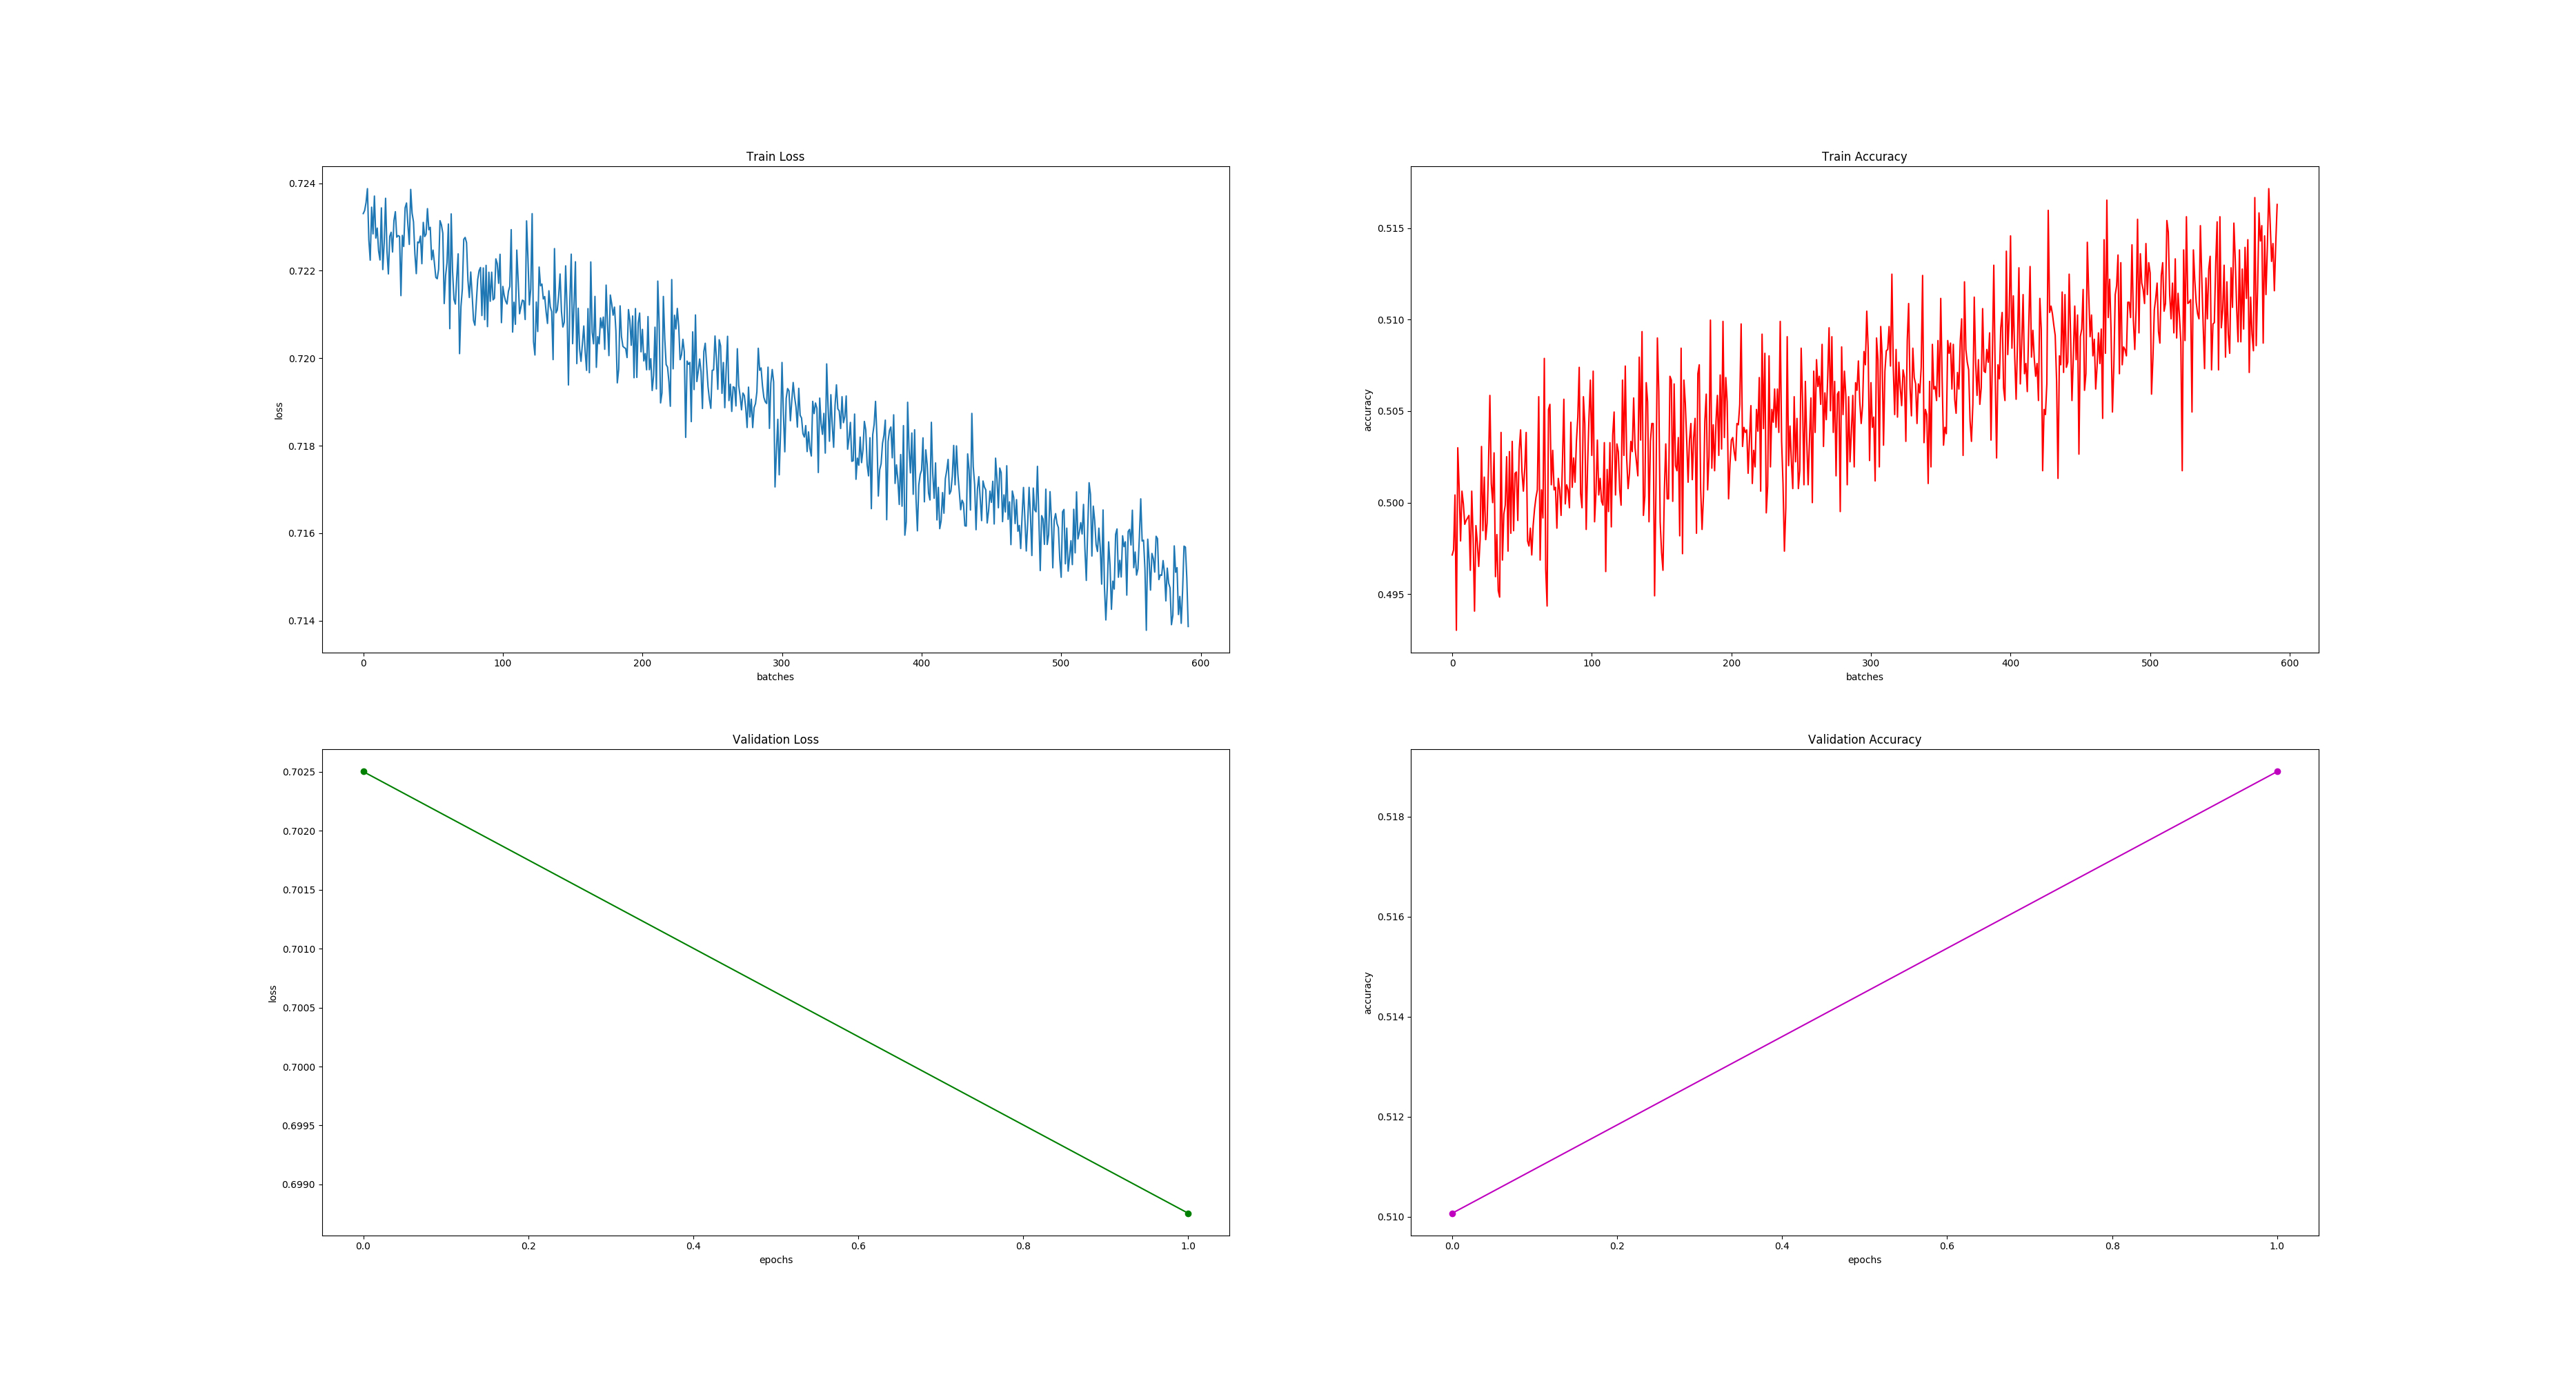
\includegraphics[width=1\textwidth]{2ep_64btch_sgd_softmax.png}
\caption{2 epochs, 64 batch-size, Softmax activation function, SGD optimizer}
\end{figure}

The mean-f1 score of the above configuration is 0.86919. Because of the reasons that we explained for the \textit{Figure 4}, we did not use this configuration either.

\begin{figure}[H]
\centering
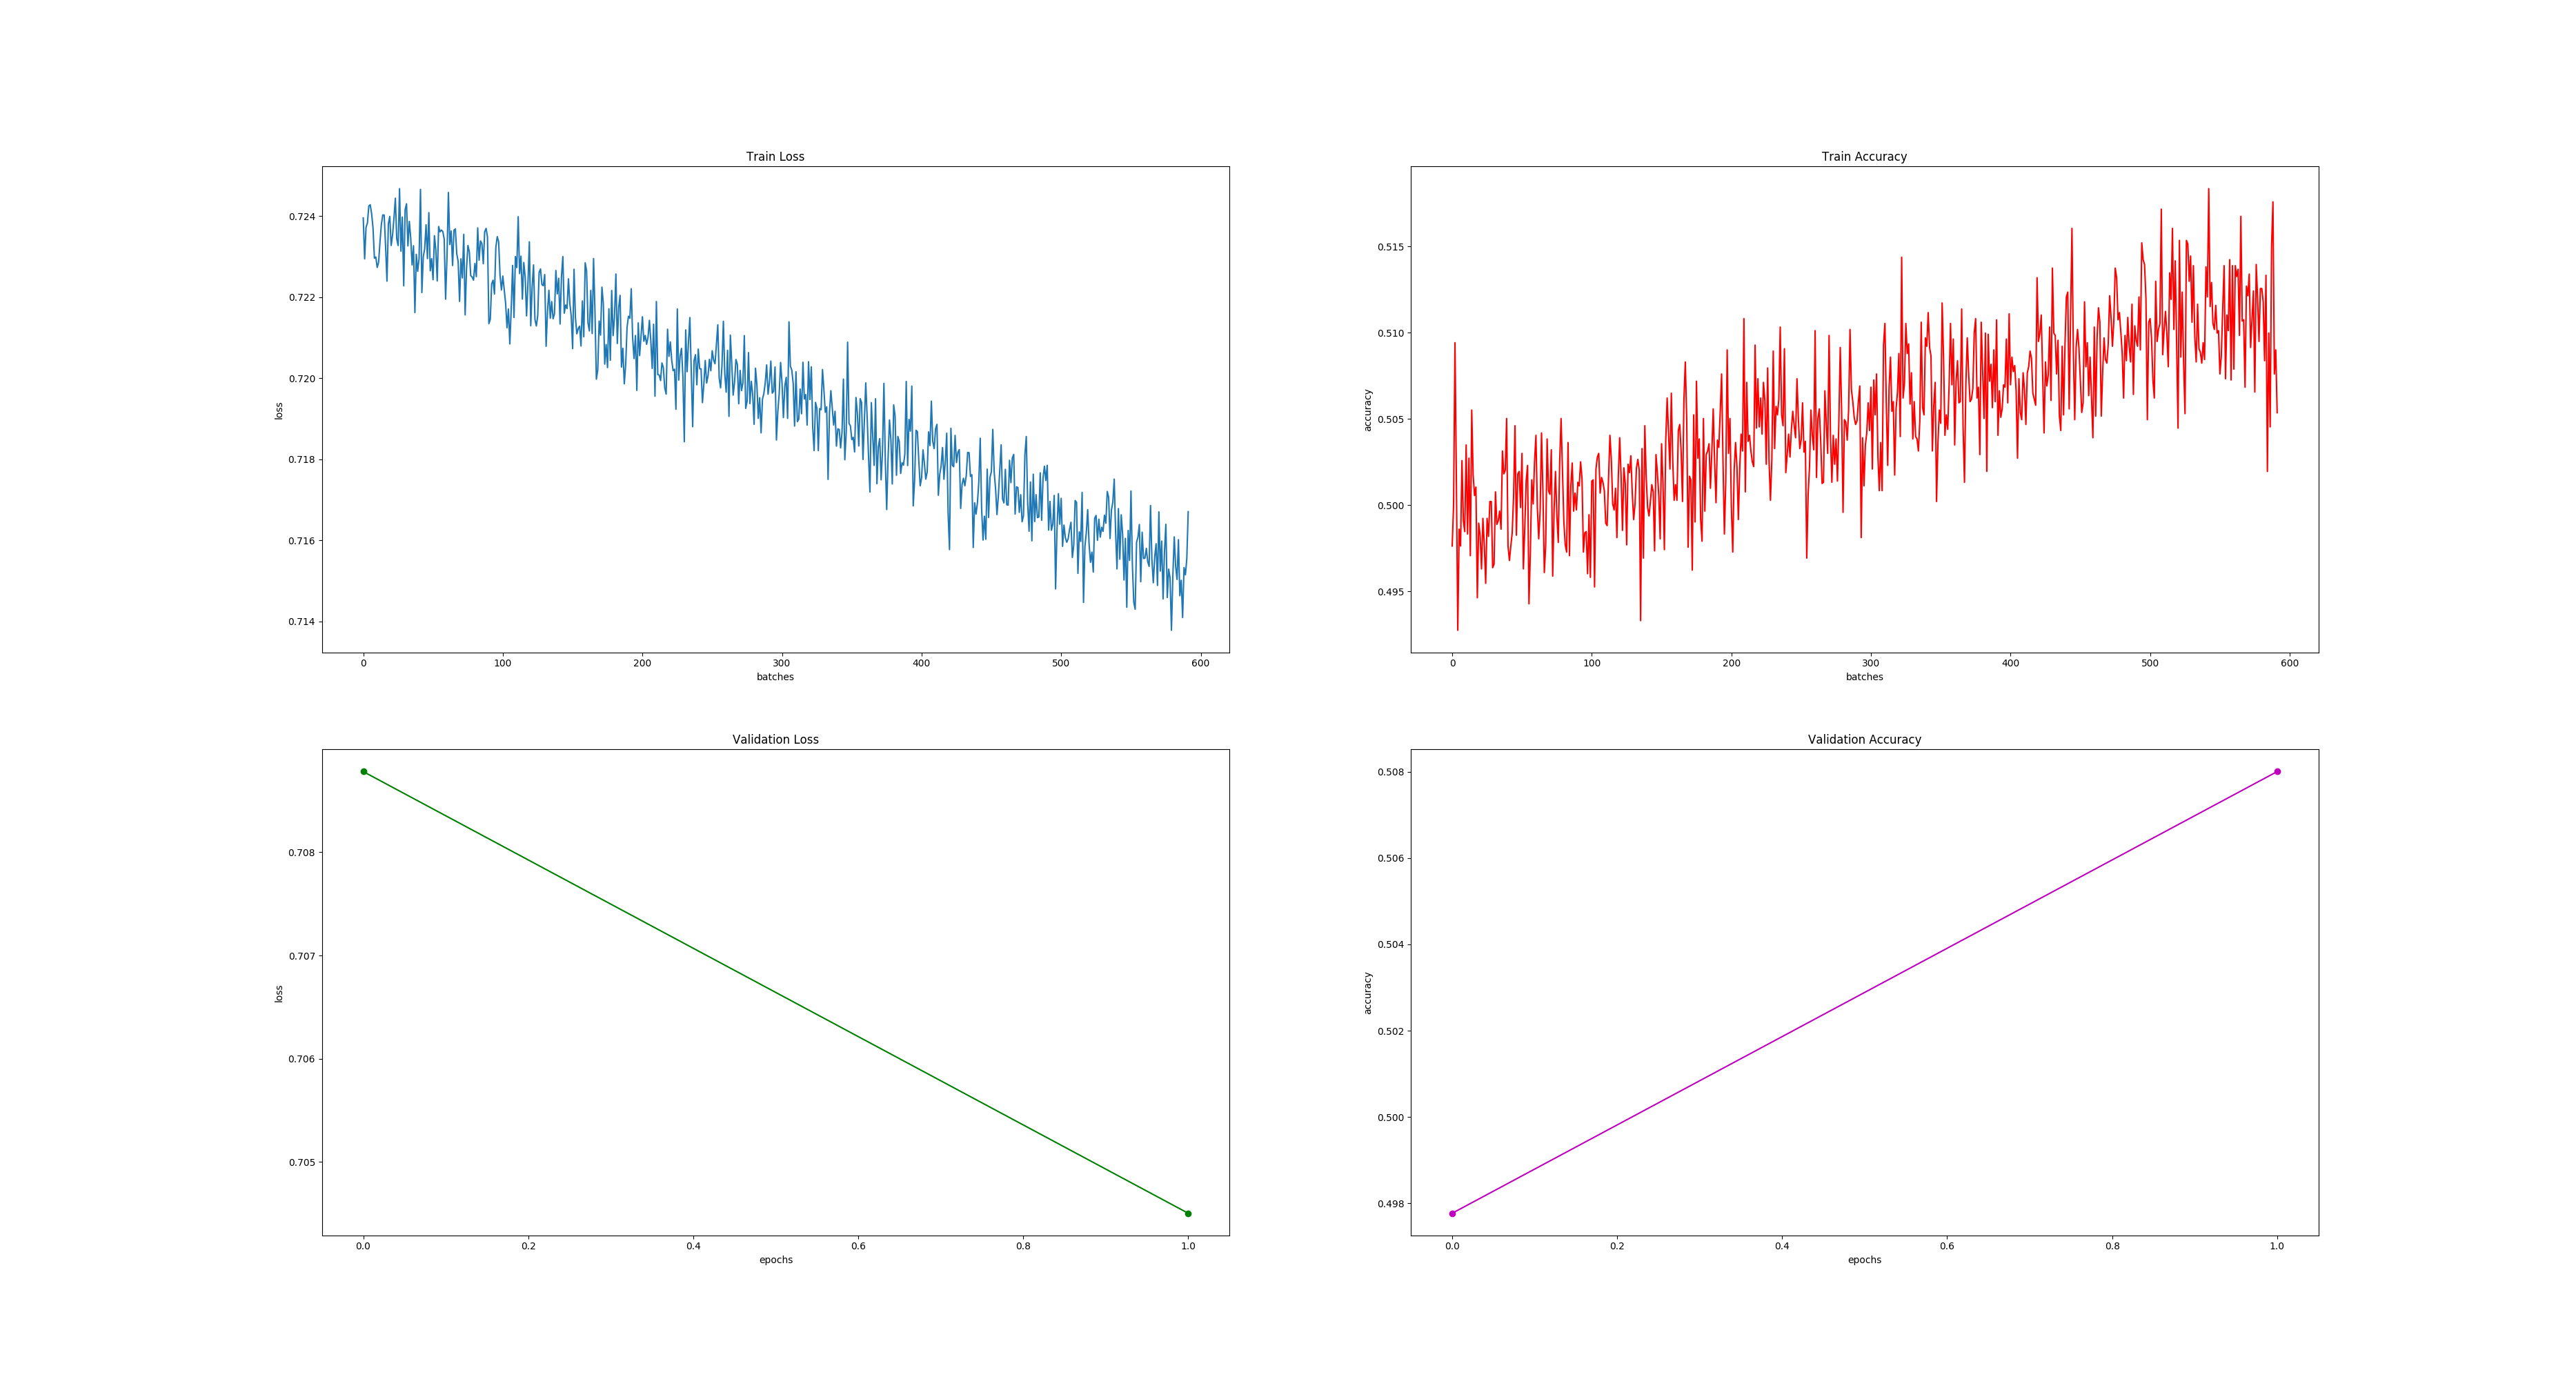
\includegraphics[width=1\textwidth]{2ep_64btch_sgd_sigmoid.png}
\caption{2 epochs, 64 batch-size, Sigmoid activation function, SGD optimizer}
\end{figure}

In contrast to \textit{Softmax} configurations, when we use the \textit{Sigmoid} as the activation function, the probabilities become higher. On the above configuration, the probabilities was clustered above 90\%. So when we threshold them, we got lots of unrelated labels. Because of this, the mean-f1 score of the above configuration is 0.06111.

\begin{figure}[H]
\centering
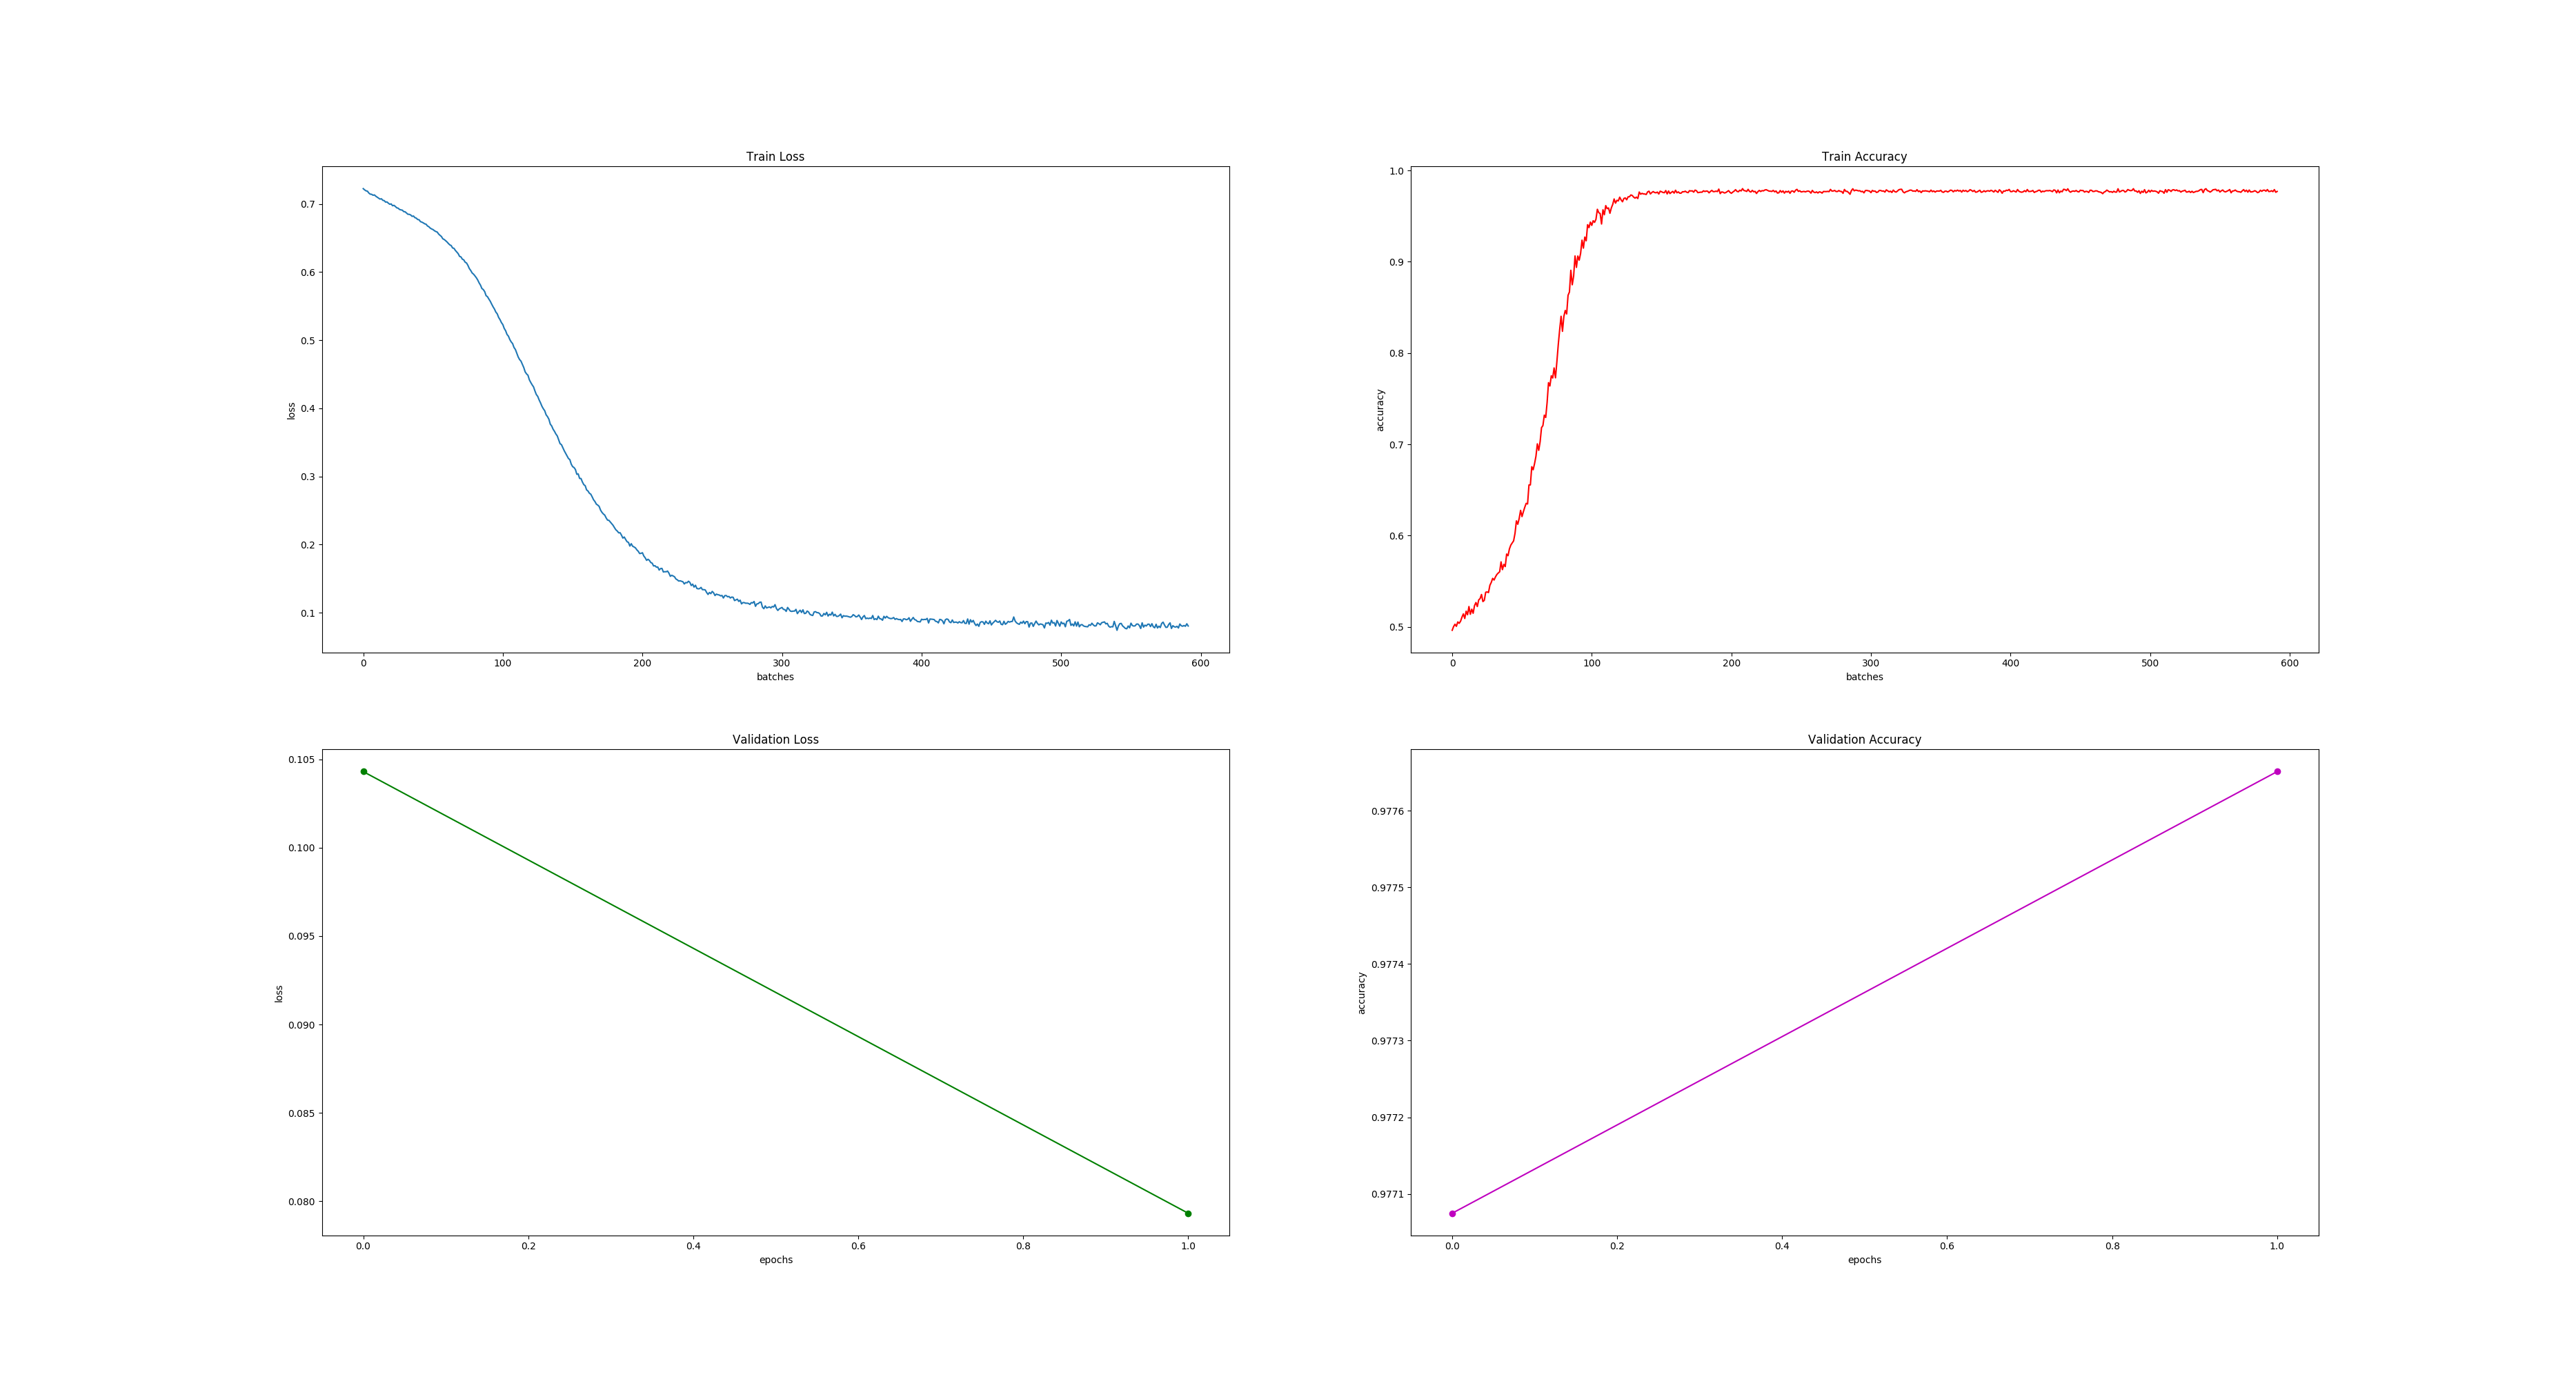
\includegraphics[width=1\textwidth]{2ep_64btch_sigmoid.png}
\caption{2 epochs, 64 batch-size, Sigmoid activation function, Adam optimizer}
\end{figure}

We achieved the best results with the above configuration. The probabilities were not clustered around some value so, we could easily threshold them. Also, the curves of the training metrics became smoother. The mean-f1 score for this configuration is 0.91488.

\section{Discussion}
Extracting training and test location vectors once and putting the results into a file saves performance and memory space. The only disadvantage of this method is that when a new data arrives, it is necessary to extract the vectors again from images and put them back into the file.\\

Using Multilayer Perceptron for training and testing has also helped to save performance and memory space. The reason of not doing training and testing Convolutional Neural Network in this homework is that it takes a very long time and does not provide multi-labels. In case of multiple labeling, a new model had to be created and trained accordingly.So we used Multilayer Perceptron. However, if testing and training were done with CNN, little better results could be obtained. Addition to these, for CNN training each image needs to be categorized according their labels. For example; in images folder, there should be dress, shirt, shoes folders and in these folders there should be images. This operation is very challenging and need too much space in memory.\\

In the training dataset, there were some pictures that were not related to the project topic. This situation were disadvantage for us. To improve the project, the data set can make better for the future.\\

We also couldn't use all images of dataset because of the memory issues. We seperated 21.000 images for training, \%10 of them as validation image, and remaining 4.000 of images didn't used. We could use libraries such as \textit{hdf5} to handle this issue but the research process took long time for us.  


\section{References}

\begin{itemize}
\item {https://keras.io/applications/}
\item {https://github.com/keras-team/keras/issues/741}
\item {https://keras.io/getting-started/sequential-model-guide/}
\item {https://www.kaggle.com/c/imaterialist-challenge-fashion-2018/discussion}
\item {https://www.safaribooksonline.com/library/view/getting-started with/9781\\786468574/ch04s04.html}
\item {https://medium.com/\@franky07724\_57962/using-keras-pre-trained-models-for-\\feature-extraction-in-image-clustering-a142c6cdf5b1}
\end{itemize}






\end{document}